\documentclass[12pt,a4paper,oneside]{article}

\usepackage[utf8]{inputenc}
\usepackage[portuguese]{babel}
\usepackage[T1]{fontenc}
\usepackage{amsmath}
\usepackage{amsfonts}
\usepackage{amssymb}
\usepackage{graphicx}
\usepackage{xcolor}
\usepackage{multicol}
\usepackage{tikz}
\usetikzlibrary{automata,positioning}

% Definindo novas cores
\definecolor{verde}{rgb}{0.25,0.5,0.35}

\author{\\Universidade Federal de Goiás (UFG) - Regional  Jataí\\Bacharelado em Ciência da Computação \\Linguagens Formais e Autômatos \\Esdras Lins Bispo Jr.}

\date{12 de dezembro de 2017}

\title{\sc \huge Terceiro Teste}

\begin{document}

\maketitle

{\bf ORIENTAÇÕES PARA A RESOLUÇÃO}

\small
 
\begin{itemize}
	\item A avaliação é individual, sem consulta;
	\item A pontuação máxima desta avaliação é 10,0 (dez) pontos, sendo uma das 06 (seis) componentes que formarão a média final da disciplina: quatro testes, uma prova e exercícios-bônus;
	\item A média final ($MF$) será calculada assim como se segue
	\begin{eqnarray}
		MF & = & MIN(10, S) \nonumber \\
		S & = & (\sum_{i=1}^{4} 0,2.T_i ) + 0,2.P  + EB\nonumber
	\end{eqnarray}
	em que 
	\begin{itemize}
		\item $S$ é o somatório da pontuação de todas as avaliações,
		\item $T_i$ é a pontuação obtida no teste $i$,
		\item $P$ é a pontuação obtida na prova, e
		\item $EB$ é a pontuação total dos exercícios-bônus.
	\end{itemize}
	\item O conteúdo exigido desta avaliação compreende o seguinte ponto apresentado no Plano de Ensino da disciplina: (2) Autômatos Finitos Determinísticos, (3) Autômatos Finitos Não-Determinísticos, e (4) Expressões Regulares.
\end{itemize}

\begin{center}
	\fbox{\large Nome: \hspace{10cm}}
\end{center}

\newpage

\begin{enumerate}
	
	\section*{Terceiro Teste}
	
	\item (5,0 pt) {\bf [Sipser 1.21 (b)]} Utilizando AFNGs, encontre a expressão regular que gera a linguagem reconhecida pelo AFN abaixo.
		\begin{center}
			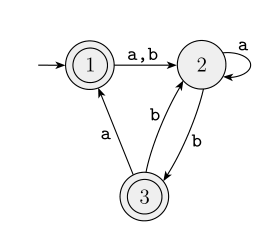
\includegraphics[width=.5\textwidth]{images/afn}
		\end{center}
	
	\vspace*{0.3cm}
	
	{\color{blue}
		{\bf Passo 1:} Criação do AFNG equivalente.
		
		\begin{tikzpicture}
			[shorten >=1pt,node distance=3cm,on grid,auto] 
			\node[state,initial] (q_0)   {$q_{ini}$}; 
			\node[state] (1) [right=of q_0] {1}; 
			\node[state] (2) [below=of 1] {2}; 
			\node[state](3) [right=of 2] {3};
			\node[state, accepting](q_f) [right=of 1] {$q_f$};
			\path[->] 
			(q_0) 	edge  [bend left] node {$\epsilon$} (1)
			(1) 	edge  [bend left] node {$\epsilon$} (q_f)
					edge  [bend right] node {$a,b$} (2)
			(2) 	edge  [bend left] node {$b$} (3)
					edge  [loop left] node {a} ()
			(3) 	edge  [bend right] node {$a$} (1)
					edge  [bend left] node {$b$} (2)
					edge  [bend right] node {$\epsilon$} (q_f)
			
			;
		\end{tikzpicture}
		
		{\bf Passo 2:} Remoção do estado 1.
		
		\begin{tikzpicture}
		[shorten >=1pt,node distance=3.5cm,on grid,auto] 
		\node[state,initial] (q_0)   {$q_{ini}$}; 
		\node[state] (2) [right=of q_0] {2}; 
		\node[state](3) [right=of 2] {3};
		\node[state, accepting](q_f) [right=of 3] {$q_f$};
		\path[->] 
		(q_0) 	edge  [bend right] node {$a,b$} (2)
			 	edge  [bend left] node {$\epsilon$} (q_f)
		(2) 	edge  [bend left] node {$b$} (3)
				edge  [loop above] node {a} ()
		(3) 	edge  [bend left] node {$b \cup a(a \cup b)$} (2)
				edge  [bend right] node {$a \cup \epsilon$} (q_f)
		
		;
		\end{tikzpicture}
		
		{\bf Passo 3:} Remoção do estado 2.
		
		\begin{tikzpicture}
		[shorten >=1pt,node distance=3.5cm,on grid,auto] 
		\node[state,initial] (q_0)   {$q_{ini}$};  
		\node[state](3) [right=of q_0] {3};
		\node[state, accepting](q_f) [right=of 3] {$q_f$};
		\path[->] 
		(q_0) 	edge  [bend right] node {$(a \cup b)a^*b$} (3)
				edge  [bend left] node {$\epsilon$} (q_f)
		(3) 	edge  [bend right] node {$a \cup \epsilon$} (q_f)
				edge  [loop below] node {$\left[b \cup a(a \cup b)\right]a^*b$} ()
		;
		\end{tikzpicture}
		
		
		
		{\bf Passo 4:} Remoção do estado 3.
		
		\begin{tikzpicture}
		[shorten >=1pt,node distance=3.5cm,on grid,auto] 
		\node[state,initial] (q_0)   {$q_{ini}$}; 
		\node[state, accepting](q_f) [right=of 3] {$q_f$};
		\path[->] 
		(q_0) 	edge  [bend left] node {$\epsilon \cup (a \cup b)a^*b(\left[b \cup a(a \cup b)\right]a^*b)^*(a \cup \epsilon)$} (q_f)
		;
		\end{tikzpicture}
		}
	
	\item (5,0 pt) Utilizando expressão regular, mostre que a classe de linguagens regulares é fechada sobre a operação de concatenação.	
	
	\vspace*{0.3cm}
	
	{\color{blue}
		{\bf Prova:} Sejam $A$ e $B$ duas linguagens regulares quaisquer. Como $A$ e $B$ são regulares, então existe as expressões regulares (ERs) $R_A$ e $R_B$ que a geram, respectivamente. Pela definição indutiva de ER, se $R_A$ e $R_B$ são ERs, então $R_A \circ R_B$ é uma ER. Como toda ER gera uma linguagem regular, $R_A \circ R_B$ é regular. Logo, a classe de linguagens regulares é fechada sob a operação de concatenação $\blacksquare$
	}

\end{enumerate}

\end{document}